\section{Preprocessing}

These are the steps we followed to carry out the preprocessing of the data. The goal of this stage is to clean, transform, and prepare the dataset, ensuring that it is consistent, reliable, and ready for the subsequent data mining tasks.

\subsection{Step 1: Getting data}
The source of the dataset used in our project comes from kaggle.com, an online platform that provides datasets, competitions, and tools for data science and machine learning. Our dataset focuses on marketing data, which will be analyzed to extract valuable insights.

\subsection{Step 2: Visualizing data}
To visualize our data, we represented it using different types of graphs, in addition to the metadata from the previous section.

\subsection{Step 3: Filtering variables selection}

 To make them easier to see and understand, we had to transform or rename a lot of variables.\\

- Age Calculation: ifood\$Age <- 2020 - ifood\$Year\_Birth creates a new column Age by subtracting the Year\_Birth from the year 2020. The original Year\_Birth column is then dropped to avoid data redundancy.\\
- Days as a Customer: ifood\$CustDays <- as.numeric(reference\_date - as.Date(ifood\$Dt\_Customer, format="\%Y-\%m-\%d")) calculates the number of days a customer has been registered. It subtracts the customer's registration date (Dt\_Customer) from a set reference\_date (December 31, 2020), converting a date variable into a useful numerical one. The original Dt\_Customer column is also removed.\\

Finally, we shortened most variable names to make them easier to represent in graphs, tables, etc.

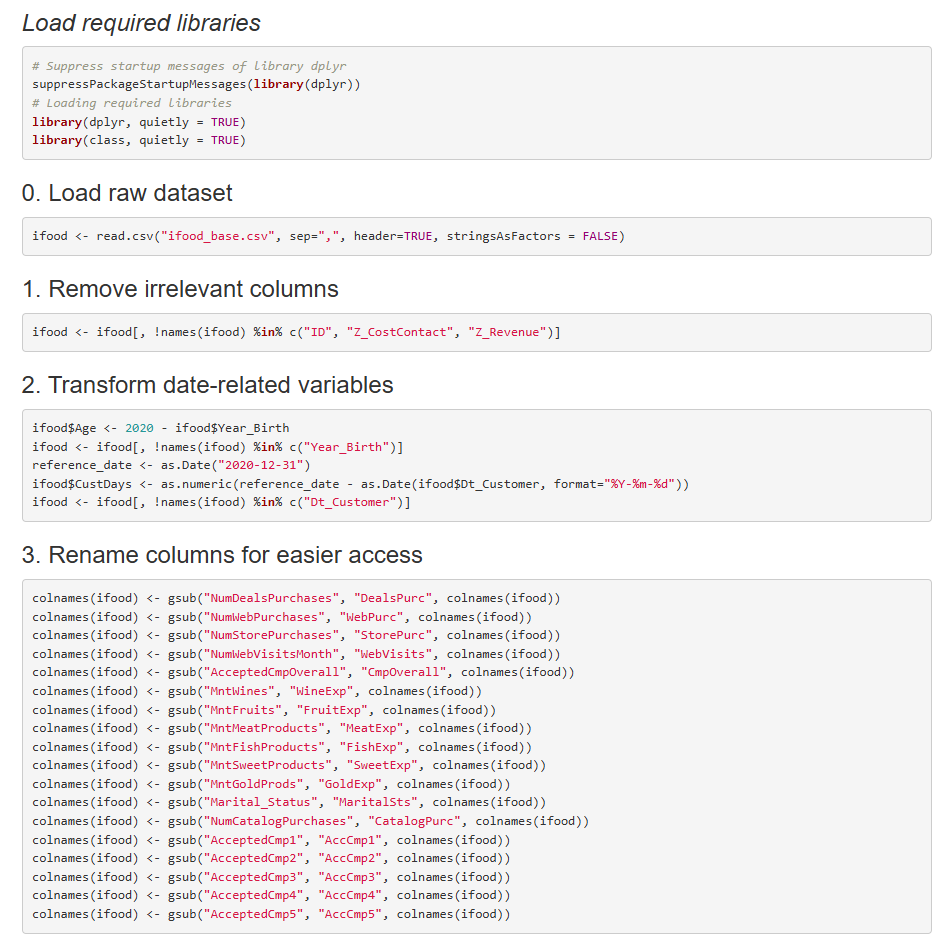
\includegraphics[width=\textwidth]{Imatges/pre1.png}

\subsection{Step 4: Missing detection and treatment}
During the preprocessing stage, we identified missing or inconsistent values by visually exploring the data to detect anomalies. For instance, in the variable Marital\_Status we found incorrect responses such as 'YOLO' and 'Absurd', which we removed to ensure data consistency.\\

Due to the fact that the Income cannot be less than 12500, we have had to impute the missing values using the KNN method.\\

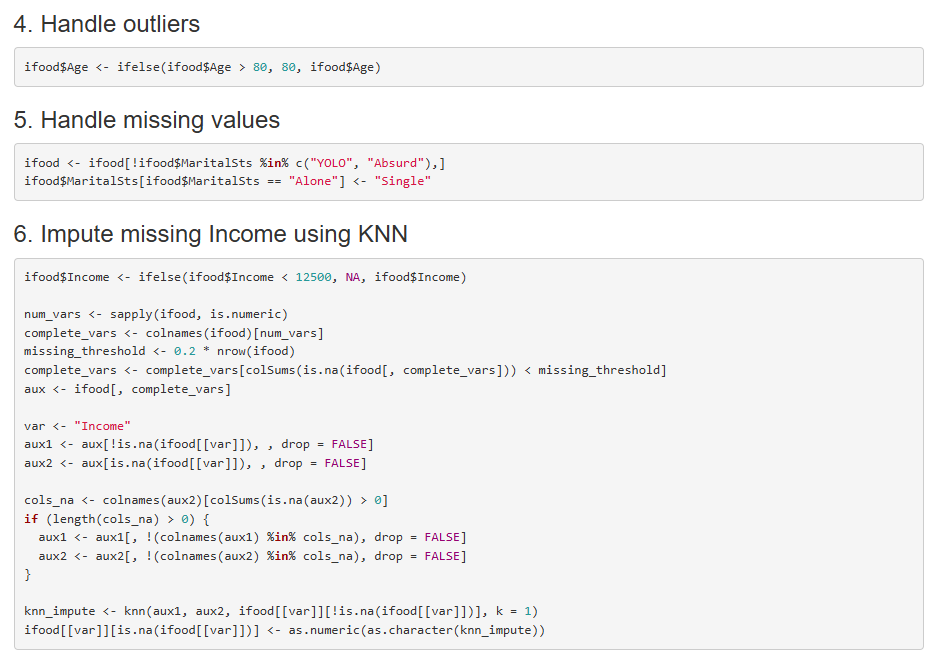
\includegraphics[width=\textwidth]{Imatges/pre2.png}
\subsection{Step 5: Outlier detection and treatment}
To handle the outliers with older people, we decided to set a limit of 80 years for individuals, so that anyone older than that age is included in the 80-year-old group.

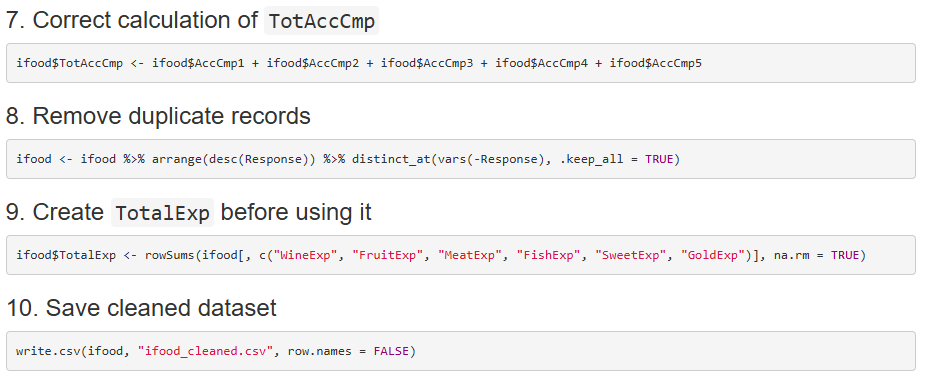
\includegraphics[width=\textwidth]{Imatges/pre3.png}
\subsection{Step 6: Feature selection}
 To clean our variables we decided to remove irrelevant columns:\\
 - ID: The ID column is a unique identifier for each record. It does'nt provide predictive value or relevant information about customer behavior or characteristics.\\
 - Z\_CostContact and Z\_Revenue: Columns starting with the letter 'Z' are often metadata variables used internally in a database, usually represents auxiliary metrics or internal calculations that are not useful for predictive analysis. In this case, both are synthetic or aggregated variables, likely related to internal company costs and revenues, which are not relevant to understanding customer behavior. \\
 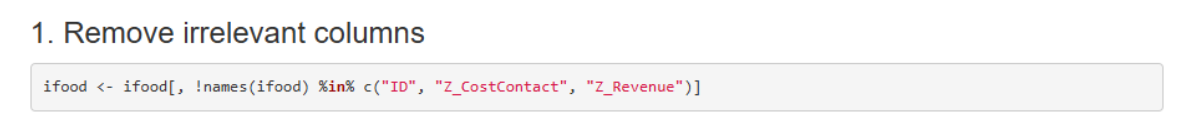
\includegraphics[width=\textwidth]{Imatges/pre8.png}
\subsection{Step 7: Transformation and new variables}
These are the new variables we have created or modified from the existing ones to obtain new information.\\
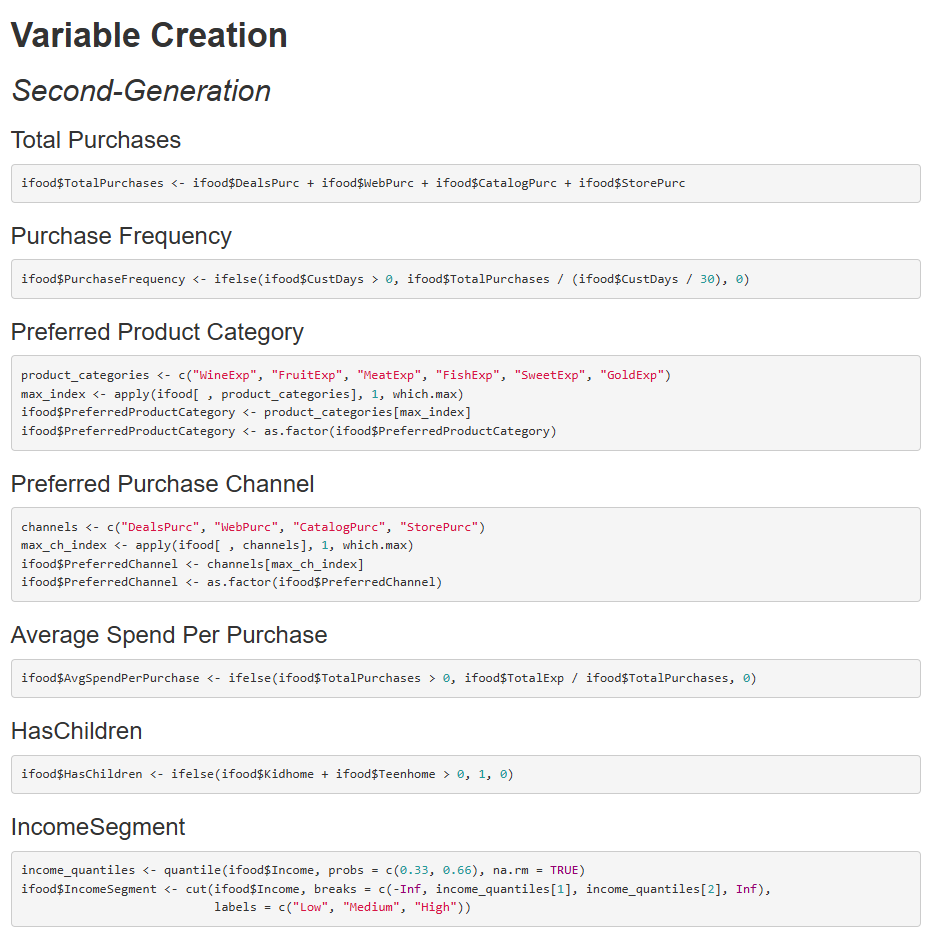
\includegraphics[width=\textwidth]{Imatges/pre4.png}

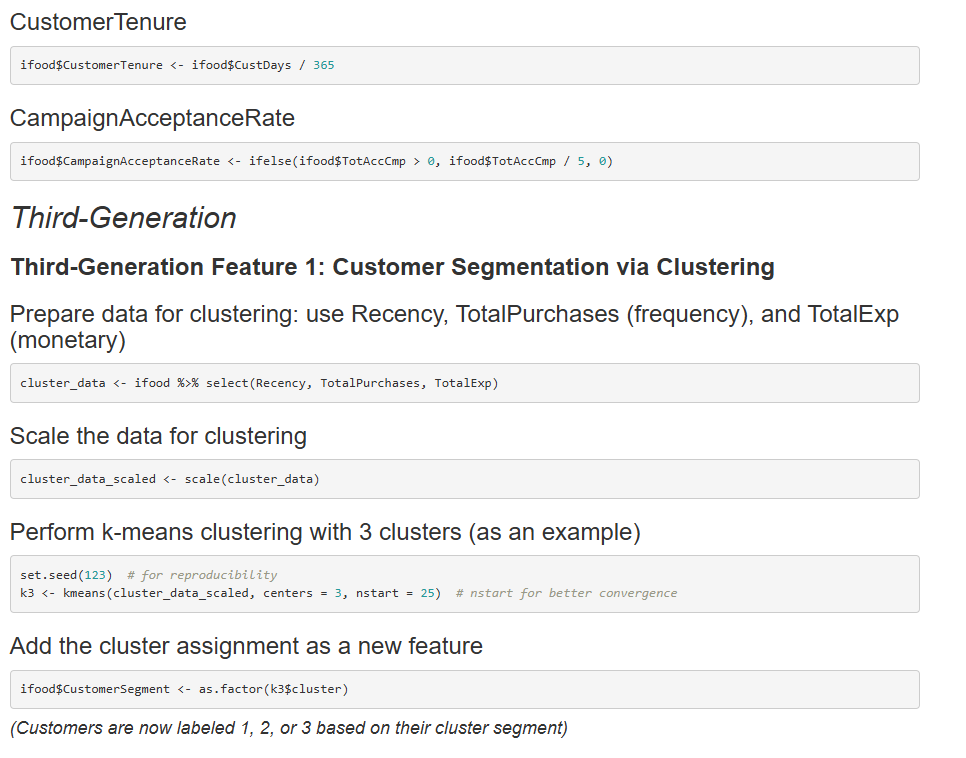
\includegraphics[width=\textwidth]{Imatges/pre5.png}
\centering
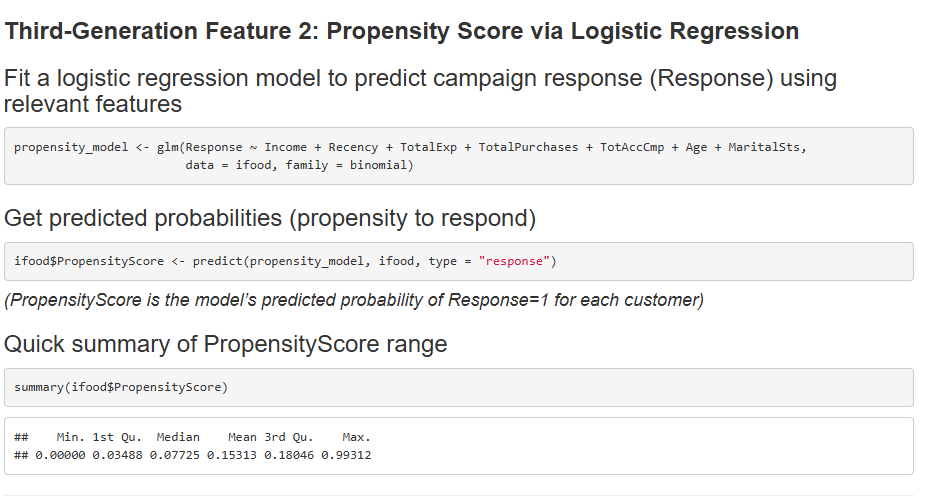
\includegraphics[width=\textwidth]{Imatges/pre6.png}
\centering
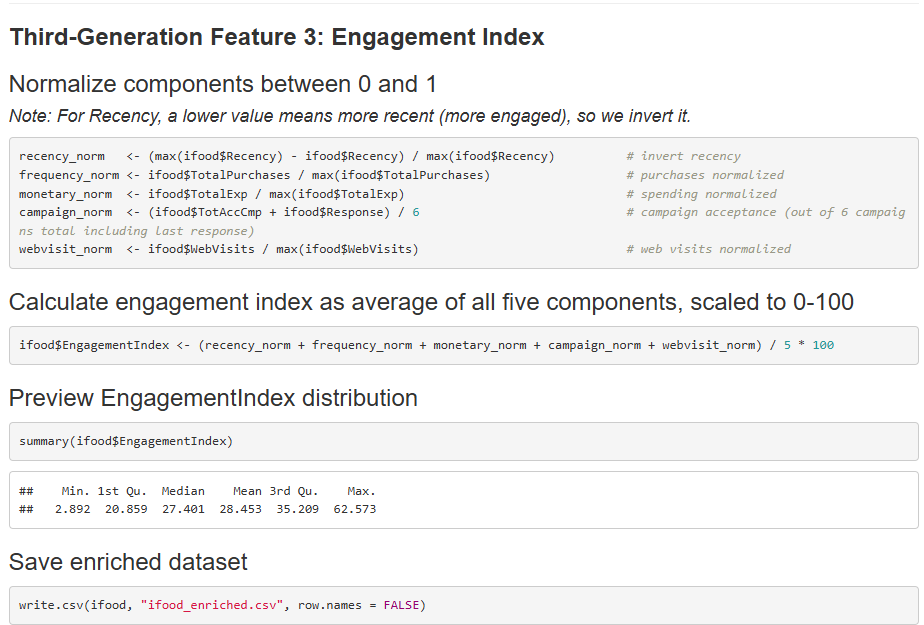
\includegraphics[width=\textwidth]{Imatges/pre7.png}
